% TODO go back and rewrite the abstract
% TODO write equations for distance metric
% TODO write equations for majority metric

\documentclass{report}
\usepackage[utf8]{inputenc}
\usepackage{cite}
\usepackage{amsfonts}
\usepackage{amsmath}
\usepackage{algorithm, algpseudocode}
\usepackage{hyperref}
\usepackage{amssymb}
\usepackage{graphicx}
\graphicspath{{../pdf/}{D:}}


\title{Restaurant Recommendations using Collaborative Filtering}
\date{December\\ 2018}
\author{Michael Siem \\ \href{mailto:siem@wisc.edu}{siem@wisc.edu}
	\and Nathan Weinshenker \\ \href{mailto:nweinshenker@wisc.edu}{nweinshenker@wisc.edu}
	\and Jack Long \\ \href{mailto:jlong25@wisc.edu}{jlong25@wisc.edu}}

\begin{document}

\maketitle

\section*{Abstract}
With the growth of ecommerce and internet, predictions of user preferences is a hot topic in todays Machine Learning community. Our goal is to use Yelp's open data set \href {https://www.yelp.com/dataset/challenge} {Yelp Dataset Challenge} as prediction measurement of potential restaurants reviewers. We will go into depth on the implementation of k Nearest Neighbors for building a recommendation system for users of similar preferences.  

\section*{Background Information}

Recommendation systems are a vital tool for providing users with personalized suggestions for items such as movies, music, and restaurants.
Product review data is widely accessible on services such as Spotify, Amazon, and Yelp.
There are two approaches that can be used to make recommendations to users based on this data, memory based, and model based.
Model based systems rely on approximating the data and determining features that are most likely to influence a users rating on an item. 
Matrix Decomposition methods such a SVD are an example of a model based system used to provide recommendations.
Over time models can become outdated and need to be updated to provide a more accurate recommendation.
Memory based systems rely upon maintaining data and finding users or items that are similar to each other.
The advantage of a memory based system is it doesn't learn a model or make any assumptions about the data so if trends change the recommendation system will adapt.
Memory based systems can do a user-user comparison or and item-item comparison.
In the user-user comparison, a user is compared to other users that have rated an item and in the item-item comparison, an item is compared to other items a user has rated to predict the rating the user will give it.
We will further study a memory based recommendation systems, K Nearest Neighbors.
\cite{5}.
	
\subsection*{K Nearest Neighbors}
	
K Nearest Neighbors (k-NN) is a memory based collaborative filter that relies upon comparing features of a user or item to other users or items to receive a recommendation. 
k-NN is also a \textbf{non-parametric} learning algorithm. What non-parametric means is that k-NN has little or no prior knowledge about the data distribution. k-NN  builds the model structure based on the training data and this allows the algorithm to be highly versatile and simple to implement with little to no information about the data \cite{3}. 

\subsubsection*{History of Nearest Neighbors}

In 1992, Paul Resnick and fellow researchers at the University of Minnesota first studied collaborative filtering systems through the GroupLens project\cite{2}\cite{8}.  Collaborative filtering began to arise as a solution for dealing with overload in online information spaces. The first collaborative filtering system was Tapestry: it allowed the user to query for
items in an information domain, such as corporate e-mail, based on
other users’ opinions or actions\cite{6}. With the growth of the Internet, collaborative filters systems have grown in scope and popularity with big name tech companies like Netflix, Amazon, and Yahoo. Today, collaborative filtering systems are used by many companies to shift through the mountains of readily available data.

\subsubsection{Nearest Neighbor Classification Derivation}
To understand k-NN, some necessary background information is required in probability. Here are some basic probability definitions . \cite{4}
\begin{enumerate}
	\item P(A $|$ B), the conditional probability, is the probability of A given B
\end{enumerate}
Now for performing k-\textbf{nearest neighbor classification }  lets assume X = training data; Y = class labels of X; and x = unknown sample.
\newline \newline
First, we will need to define our distance metric 
Let $d$ be a distance measure (using euclidean distance)for our dataset $D$ where
\begin{equation}
d= \sqrt{(x_{i1} - x_{j1})^2 + (x_{i2} - x_{j2})^2 + ... + (x_{ip} - x_{jp})^2}
\end{equation}
\begin{equation}
D = (x_{1}, y_{1}), (x_{2}, y_{2}), ... , (x_{n}, y_{n})
\end{equation}
Secondly, we need to sort all the distances for our set D , i.e,
\begin{equation}
d(x,x_{i}) <= d(x,x_{i+1})
\end{equation}

The first k $\epsilon$ N points (where N is set of closest distances) follow this  enumeration 
\begin{equation}
N_{k}(x) = (x_{1}, y_{1}), (x_{2}, y_{2}), ... , (x_{k}, y_{k}) 
\end{equation} 
\textsubscript{this is called a k-neighborhood of x (in D)}. \newline\newline
We will now define our classifier as 
\begin{equation}
\hat{p}(Y = y | x) = \frac{1}{k} \sum_{x',y' \epsilon N_{k}(x) }  I(y = y')
\end{equation}
and then we will predict the class of a user using the maximal predicted probability.
\begin{equation}
\hat{Y}(x) = argmin_{y \epsilon Y} \hat{p}(Y = y |x)
\end{equation}
\textsubscript{i.e., the majority class with repect to the classes of the neighbors}. \newline\newline

\subsubsection*{Classification Decision Rule}
With defining our distance metric and classification rule, we can now test it's classification.
With 1-nearest neighbor rule, the predicted class of test sample x is set equal to the true class y of its nearest neighbor, where $mi$ is a nearest neighbor to x if the distance \cite{7}.
\begin{equation}
d(m_{i},x) = min_{j}(d(m_{j},x))
\end{equation} 
Once all the test samples have been classified, the classification accuracy is based on the ratio of the number of correctly classified samples to the total number of samples classified, given in the form.
\begin{equation}
Accurary = \sum \frac{correctly classified}{total N}
\end{equation}
		


\subsubsection*{The Distance Function}

Several methods can be used to evaluate the distances between the neighbors and the point of interest.
We will first look at the use of the Euclidean distance or the straight-line distance between the points.

\begin{equation}
d(x_{i},x_{j}) = \sqrt{(x_{i1} - x_{j1})^2 + (x_{i2} - x_{j2})^2 + ... + (x_{ip} - x_{jp})^2}
\end{equation}

\subsubsection{K Nearest Neighbor Pseudocode }
\begin{algorithm}
  \caption{K Nearest Neighbour}
  \begin{algorithmic}
  	\State Classify (X,Y,x) // X:training data, Y: class labels of X, x:unknown sample
	\For{ t = 1 to T}
	\State Compute the distance between $d(X, x)$
	\State Sort all the distances in ascending order
	\EndFor
	\State Find the set Z containing indices for the k smallest distances $d(X_{i},x)$
	\State return the set of k closest points 
  \end{algorithmic}
\end{algorithm}



%Example matrix:
%			\[
%     			M=
%  				\begin{bmatrix}
%    					1 & 3 & ? & 3 & 1 \\
%    					3 & 2 & 5 & 8 & 7 \\
%    					3 & ? & 5 & ? & ? \\
%    					9 & ? & 3 & 2 & 1
%  				\end{bmatrix}
%			\]
%\textit{ where M is sparse (i.e., “with missing entries”, not “containing a lot of zeros”)}





\section*{Warm-up}
Here are a couple activites to warm up on k-NN 
\begin{enumerate}
	\item The below data are 2D points with their classification. If we were to add the point (1,1) using 3-NN (K = 3) what would be the classification of this point?
	\begin{figure}[H]
		\centering
		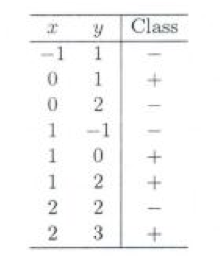
\includegraphics{image/Picture1.png}
	\end{figure}
	\item Below is a diagram of points with classifications of either Red Triangle or Blue Square. A new point is introduced as the green circle. If the correct classification of the circle is Red Triangle, what k-values would misclassify this point? What does this tell us about having too large a k value
	\begin{figure}[H]
		\centering
		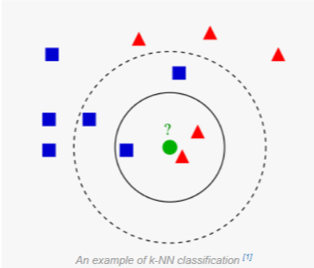
\includegraphics{image/Picture2.png}
	\end{figure}
	\item How does raising the k value affect performance in data sets with a lot of noise? 
	\item Consider taking a 2D data set and then transforming it to fit into a 3D space. How would raising the dimension of K-NN effect the accuracy of the classifier?
	\item If the Minkowski distance is defined as: 
	\begin{equation}
	D (x, y) = ((\sum_{i}^{m}| x_{i} - y_{i}|^p)^\frac{1}{p})
	\end{equation}
     then when would you use Minkowski distance over Euclidean Distance?
	

\item Draw a Voronoi diagram
\end{enumerate}

\section*{Main Activity}

The main activity will be evaluating a KNN as a restaurant recommendation system using the Yelp dataset from \href{https://www.yelp.com/dataset}{https://www.yelp.com/dataset}.
The dataset originally contains 5,996,996 reviews for 188,593 businesses in 10 metropolitan areas.
We preprocessed the data set to narrow it down to 1 restaurant with 500 reviews for the activity, therefore we will be doing a user-user comparison.  
The activity will done using the Matlab script KNN.m.

\begin{enumerate}

\item Choosing K value

\item Evaluate different distance functions

\item Evaluate different classification metrics

\end{enumerate}

%\section*{Future Work}
%When classifying users some 

\begin {thebibliography}{999}
\bibliographystyle{plain}
	\bibitem{1}
	Leif E. Peterson
	Scholarpeida
	\href{http://www.scholarpedia.org/article/K-nearest_neighbor}{Scholarpedia}
	\bibitem{2}
	Joseph A. Konstan
    University of Minnesota
    Introduction to Recommender Systems
	\href{https://www-users.cs.umn.edu/~konstan/SIGMOD-2008-Tut.pdf}{UMN SIGMOD-2008}
	\bibitem{3}
	Benjamin Soltoff
    University of Chicago
    Statistical learning: non-parametric methods MACS-3100
	\href{https://cfss.uchicago.edu/persp010_nonparametric.html#objectives}{University Chicago MACS-3100}
	\bibitem{4}
	Lars Schmidt-Thieme
	 Institute for Computer Science University of Hildesheim
	 \href{https://www.ismll.uni-hildesheim.de/lehre/ml-07w/skript/ml-2up-03-nearest-neighbor.pdf} {K-NN Derivation}
	 \bibitem{5}
	Yifei Feng and Zhengli Sun
	Stanford University 
	Yelp User Rating
	 \href{http://cs229.stanford.edu/proj2014/Yifei%20Feng,%20Zhengli%20Sun,%20Yelp%20User%20Rating%20Prediction.pdf} {Link towards paper}
	 \bibitem{6}
	Collaborative Filtering Recommender Systems
	By Michael D. Ekstrand, John T. Riedl
	and Joseph A. Konstan
	 \href{http://files.grouplens.org/papers/FnT%20CF%20Recsys%20Survey.pdf} {Group Lens}
	 \bibitem{7}
	 R. Nowak
	 University of Wisconsin-Madison
	 ECE 830 Fall 2010 Statistical Signal Processing
	 \href{http://nowak.ece.wisc.edu/ece830/ece830_lecture24.pdf}{Signal Processing}
	 \bibitem{8}
	 Paul Resnick
	 MIT Coordination Center for Science
	 GroupLens: An Open Architecture for Collaborative
Filtering of Netnews
	\href{http://delivery.acm.org/10.1145/200000/192905/p175-resnick.pdf?ip=72.33.2.208&id=192905&acc=PUBLIC&key=066E7B0AFE2DCD37%2E4D4702B0C3E38B35%2E4D4702B0C3E38B35%2E4D4702B0C3E38B35&__acm__=1544639596_64ed1d6ccc2584122e84fe8f012afa64}{Collborative Filtering}
\end{thebibliography}
\end{document}


